\documentclass[a4paper,titlepage,12pt]{article}
\usepackage[utf8]{inputenc} %Make sure all UTF8 characters work in the document
\usepackage{listings} %Add code sections
\usepackage{color}
\usepackage{graphicx}
\usepackage{titling}
\usepackage{textcomp}
\usepackage{tabularx}
\usepackage[hyphens]{url}
\usepackage[bottom]{footmisc}
\usepackage[yyyymmdd]{datetime}
\definecolor{listinggray}{gray}{0.9}
\definecolor{lbcolor}{rgb}{0.9,0.9,0.9}
\usepackage{longtable}

%Set page size
\usepackage{geometry}
\geometry{margin=3cm}
\usepackage{parskip} 

\renewcommand{\dateseparator}{-}

%\author{
%    Emil Segerbäck - emise935
%    \and
%    Frans Skarman - frask812
%    \and
%    Hannes Tuhkala - hantu447
%    \and
%    Malcolm Vigren - malvi108
%    \and
%    Noak Ringman - noari093
%    \and
%    Olav Övrebö - olaov121
%    \and
%    Robin Sliwa - robsl733}


%%%%%%%%%%%%%%%%%%%%%%%%%%%%%%%
% Header and footer
%%%%%%%%%%%%%%%%%%%%%%%%%%%%%%%
\usepackage{fancyhdr}
\pagestyle{fancy}

\lhead{
	
\includegraphics[width=0.15\linewidth]{images/logo_full.png}
	}
\chead{LiTHe Hex}
\rhead{\today}
\setlength\headheight{26pt} 

\lfoot{TSEA29 - KMM \\ LIPS Kravspecifikation}
\rfoot{Grupp 9}


\title{\textbf{Kravspecifikation}}
\date{\today}

\newcounter{reqNr}
\setcounter{reqNr}{0}
\newcommand{\nextReqNr}{\stepcounter{reqNr}\arabic{reqNr}}

\begin{document}
	\maketitle
	\newpage

	
	\begin{center}

		%%%%%%%%%%%%%%%%%%%%%%%%%%%%%%%%%%%%%%%%%%%%%%%%%%%%%%%%%%%%%%%%%%%%%%%%%%%%%%%%%
		%						Medlemmar
		%%%%%%%%%%%%%%%%%%%%%%%%%%%%%%%%%%%%%%%%%%%%%%%%%%%%%%%%%%%%%%%%%%%%%%%%%%%%%%%%%

		\section*{Projektidentitet}
		Grupp 9, Ht 2016, LiTHe Hex

		Linköpings Tekniska Högskola, ISY

		\begin{table}[h]
			\begin{tabular}[pos]{| l | l | l | l |}
				\hline
				\textbf{Namn} & \textbf{Ansvar} & \textbf{Telefon} & \textbf{E-post} \\ \hline
				Emil Segerbäck & & & emise935@student.liu.se \\ \hline
				Frans Skarman & Dokumentansvarig & 0708798660 & frask812@student.liu.se \\ \hline
				Hannes Tuhkala & & & hantu447@student.liu.se \\ \hline
				Malcolm Vigren & Projektledare & 0725341681 & malvi108@student.liu.se \\ \hline
				Noak Ringman &  &  & noari093@student.liu.se \\ \hline
				Olav Övrebö &  &  & olaov121@student.liu.se \\ \hline
				Robin Sliwa &  &  & robsl733@student.liu.se \\ \hline
			\end{tabular}
		\end{table}


		Kundinfo?

		\textbf{Kursansvarig}: Tomas Svensson Rum 3B:528 013-28 13 68 tomas.svensson@liu.se

		\textbf{Handledare}:


		
		\newpage


		%%%%%%%%%%%%%%%%%%%%%%%%%%%%%%%%%%%%%%%%%%%%%%%%%%%%%%%%%%%%%%%%%%%%%%%%%%%%%%%%%
		%						Historik
		%%%%%%%%%%%%%%%%%%%%%%%%%%%%%%%%%%%%%%%%%%%%%%%%%%%%%%%%%%%%%%%%%%%%%%%%%%%%%%%%%

		\section*{Dokumenthistorik}
		\begin{table}[h]
			\begin{tabular}[pos]{| l | l | l | l | l |}
				\hline
				\textbf{Version} & \textbf{Datum} & \textbf{Utförda förändringar} 
				& \textbf{Utförda av} & \textbf{Granskad} \\ \hline

				0.1 & 2016-09-05 & Första utkastet & ckr & \\ \hline

			\end{tabular}
		\end{table}

	\end{center}

	%%%%%%%%%%%%%%%%%%%%%%%%%%%%%%%%%%%%%%%%%%%%%%%%%%%%%%%%%%%%%%%%%%%%%%%%%%%%%%%%%
	%						Inledning
	%%%%%%%%%%%%%%%%%%%%%%%%%%%%%%%%%%%%%%%%%%%%%%%%%%%%%%%%%%%%%%%%%%%%%%%%%%%%%%%%%

	\newpage

	\section{Inledning}
	I detta dokument kommer det att framgå vilken funktionalitet som produkten kommer 
	att ha vid leverans. All funktionalitet har strukturerats i olika krav där det 
	blir tydligt hur vida kravet är uppfyllt eller inte. Krav har olika nivåer där
	nivå 1 är se krav som måste ha uppfyllts vid leverans. Nivå 2 ses som bör krav 
	och uppfylls i mån om tid. Varje krav kommer att ha följande struktur. 
	\textbf{fin figur}

	\subsection{Parter}
	Projektet har parter som består av beställare/kund Tomas Svensson lektor vid 
	Linköpings tekniska högskola och producent projektgrupp 9 bestående av 7 
	studenter från D-programmet vid Linköpings tekniska högskola. 
	\subsection{Syfte och mål}
	Syftet och målet med projektet är att utveckla en sexbent robot som själv
	kan navigera sig ut ur en labyrint. I labyrinten ska roboten även kunna ta 
	sig över hinder för att komma vidare. 
	\subsection{Användning}
	\textbf{text}
	\subsection{Bakgrundsinformation}
	För regler om uppbyggnad om labyrinten roboten är tänkt att ta sig igenom, se
	Bilaga A: Banregler.

	%%%%%%%%%%%%%%%%%%%%%%%%%%%%%%%%%%%%%%%%%%%%%%%%%%%%%%%%%%%%%%%%%%%%%%%%%%%%%%%%%
	%						Översikt
	%%%%%%%%%%%%%%%%%%%%%%%%%%%%%%%%%%%%%%%%%%%%%%%%%%%%%%%%%%%%%%%%%%%%%%%%%%%%%%%%%

  \newpage
	\section{Översikt av systemet}
	Systemet ska innehålla tre enheter. En centralenhet för kommunikation med en dator, en motorikenhet
	som sköter hur benen rör sig samt en sista enhet för sensorer. Centralenheten är även den enhet som
	tar beslut och kommunicerar med de andra enheterna.
	\begin{figure}[h]
		\centering
		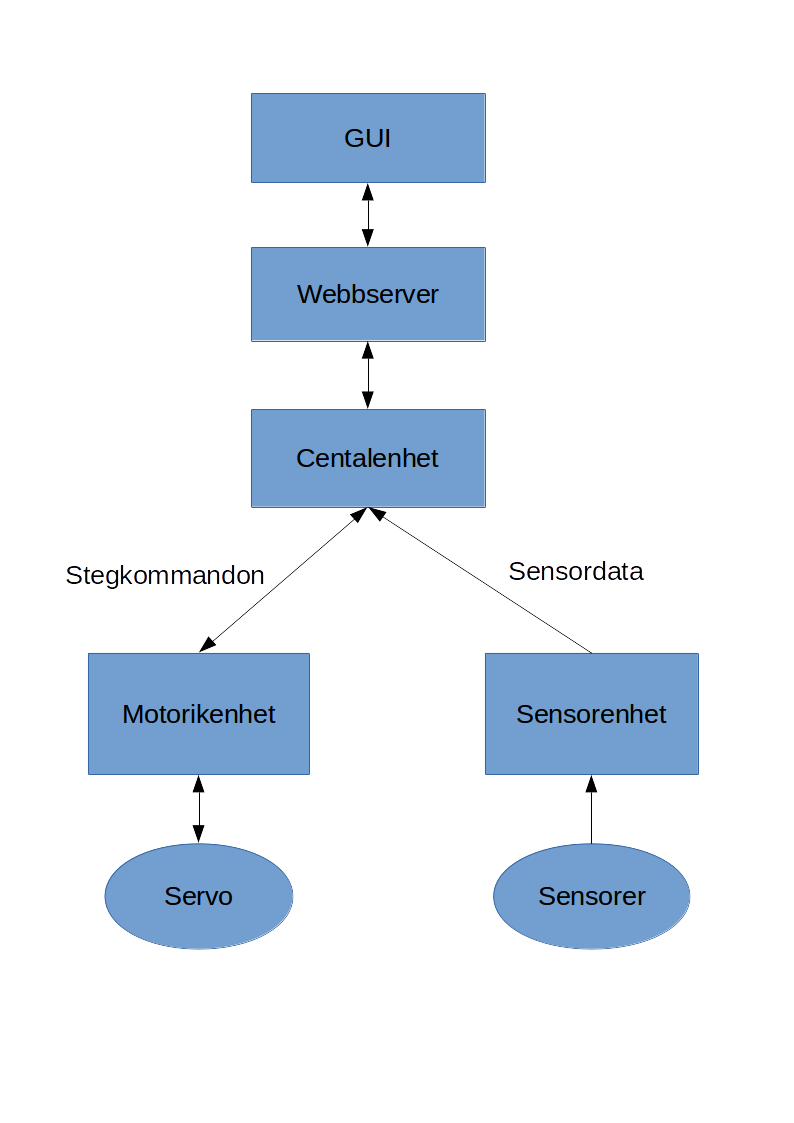
\includegraphics[width=0.5\linewidth]{images/overview.png}
		\caption{Översikt av systemet}
		\label{fig:images/overview}
	\end{figure}

	\subsection{Grov beskrivning av produkten}
	Produkten är en sexbent robot som känner av sin omgivning, och kan gå autonomt
	genom en bana samt styras manuellt.
	\subsection{Produktkomponenter}
	I leveransen ska det ingå en autonom sexbent robot med tillhörande GUI som kan användas för att 
	styra roboten manuellt. Teknisk dokumentation och demonstration ingår även. 
	\subsection{Beroenden  till andra system}
	Det beroende som finns är centralenhetens Wi-Fi-kommunikation som används för 
	att kommunicera med en dator.
	\subsection{Ingående delsystem}
    \begin{itemize}
        \item Centralenheten
        \item Motorikenheten
        \item Sensorenheten
    \end{itemize}
	\subsection{Avgränsningar}
	Roboten behöver inte klara mer avancerade former på labyrinten den beskriven i Bilaga A: Banregler.
	\subsection{Generella krav på hela systemet}

	%Generella krav på systemet
	\begin{table}[h]
		\begin{tabularx}{\textwidth}{|c|l|X|l|}
		\hline
			\textbf{Nr} & \textbf{Förändring} & \textbf{Kravtext} & \textbf{Prioritet} 
				\\ \hline
	
			\nextReqNr & Original & Roboten ska ha ett autonomt läge. & 1
					\\ \hline

			\nextReqNr & Original & Det ska finnas en knapp där man startar 
				roboten. & 1
				\\ \hline

			\nextReqNr & Original & Roboten ska kunna styras med dator 
				via WiFi-länk. & 1
				\\ \hline
		
			\nextReqNr & Original & Robotens sensordata ska gå att läsa 
				med dator via Wi-Fi & 1
				\\ \hline

			\nextReqNr & Original & Robotens styrbeslut ska gå att läsa 
				med dator via Wi-Fi & 1
				\\ \hline
		\end{tabularx}
	\end{table}

	%%%%%%%%%%%%%%%%%%%%%%%%%%%%%%%%%%%%%%%%%%%%%%%%%%%%%%%%%%%%%%%%%%%%%%%%%%%%%%%%%
	%						Centralenhet
	%%%%%%%%%%%%%%%%%%%%%%%%%%%%%%%%%%%%%%%%%%%%%%%%%%%%%%%%%%%%%%%%%%%%%%%%%%%%%%%%%
	\section{Delsystem centralenhet}
	Centralenheten ska styra alla andra delsystem i konstruktionen, samt sköta
	kommunikation till omvärlden via bland annat WiFi. Denna utgörs av en Raspberry
	Pi, som är en passande dator då den har inbyggd hårdvara för WiFi samt
	ett operativsystem, som gör att programmering kan ske på en relativt hög nivå.

	\subsection{Krav}
	\begin{table}[h]
		\label{tab:label}
		\begin{tabularx}{\textwidth}{|c|l|X|l|}
			\hline
			\textbf{Nr} & \textbf{Förändring} & \textbf{Kravtext} & \textbf{Prioritet} 
				\\ \hline

			\nextReqNr & Original & Centralenheten ska kunna kommunicera 
				med en dator via WiFi. & 1
				\\ \hline

			\nextReqNr & Original & Centralenheten ska kunna ta emot och 
				behandla data från sensorenheten.& 1
				\\ \hline

			\nextReqNr & Original & Centralenheten ska kunna ta emot, 
				behandla och skicka information till motorikenheten. & 1
				\\ \hline

			\nextReqNr & Original & Centralenheten ska kunna hålla koll 
				på positionen i labyrinten med hjälp av sensorerna. & 1
				\\ \hline

			\nextReqNr & Original & Centralenheten ska kunna upptäcka hinder. & 2
			\\ \hline

		\end{tabularx}
	\end{table}



	%%%%%%%%%%%%%%%%%%%%%%%%%%%%%%%%%%%%%%%%%%%%%%%%%%%%%%%%%%%%%%%%%%%%%%%%%%%%%%%%%
	%						Motorikenhet
	%%%%%%%%%%%%%%%%%%%%%%%%%%%%%%%%%%%%%%%%%%%%%%%%%%%%%%%%%%%%%%%%%%%%%%%%%%%%%%%%%

	\section{Delsystem motorikenhet}
	Benkontrollerns syfte är att ta data om vilket håll roboten ska gå och styra benen enligt de
	instruktionerna. Den ska bestå av en AVR-processor som tar kommandon från styrdatorn och skickar
	servopositioner till de individuella servona.

	\subsection{Krav}
	\begin{table}[h]
		\label{tab:label}
		\begin{tabularx}{\textwidth}{|c|l|X|l|}
			\hline
			\textbf{Nr} & \textbf{Förändring} & \textbf{Kravtext} & \textbf{Prioritet} 
				\\ \hline

			\nextReqNr & Original & Motorikenheten ska möjliggöra rörelse framåt och 
				bakåt samt rotation. & 1
				\\ \hline

			\nextReqNr & Original & Motorikenheten ska ge roboten två olika gånglägen,
				ett där roboten går 
				snabbt och en där roboten går med högre precision.& 2
				\\ \hline

			\nextReqNr & Original & Motorikenheten ska kunna skicka data om höjden 
				på underlaget
  				till centralenheten. & 2
				\\ \hline

			\nextReqNr & Original & Motorikenheten ska möjliggöra kliv över hinder 
				beskrivet i Bilaga A:
  				Banregler. & 2
				\\ \hline

			\nextReqNr & Original & Motorikenheten ska möjliggöra rörelse åt höger 
				och vänster. & 2 
				\\\hline

		\end{tabularx}
	\end{table}


	%%%%%%%%%%%%%%%%%%%%%%%%%%%%%%%%%%%%%%%%%%%%%%%%%%%%%%%%%%%%%%%%%%%%%%%%%%%%%%%%%
	%						Sensorer
	%%%%%%%%%%%%%%%%%%%%%%%%%%%%%%%%%%%%%%%%%%%%%%%%%%%%%%%%%%%%%%%%%%%%%%%%%%%%%%%%%
	\section{Delsystem sensorer}
	Delsystem sensorer är en mikrodator som ska läsa in data från sensorer för att sedan skicka 
	det vidare till centralenheten. Sensorer är avståndsmätare och eventuella extra sensorer 
	för att detektera hinder (exempelvis en kamera).

	\subsection{Krav}
	\begin{table}[h]
		\label{tab:label}
		\begin{tabularx}{\textwidth}{|c|l|X|l|}
			\hline
			\textbf{Nr} & \textbf{Förändring} & \textbf{Kravtext} & \textbf{Prioritet} 
				\\ \hline

			\nextReqNr & Original & Sensorenheten ska kunna tolka avstånds- mätarnas data & 1
				\\ \hline

			\nextReqNr & Original & Sensorenheten ska kunna kommunicera med 
				centralenheten. Det är tolkad data från sensorer som ska skickas.& 1
				\\ \hline

		\end{tabularx}
	\end{table}


	%%%%%%%%%%%%%%%%%%%%%%%%%%%%%%%%%%%%%%%%%%%%%%%%%%%%%%%%%%%%%%%%%%%%%%%%%%%%%%%%%
	%						Sensorer
	%%%%%%%%%%%%%%%%%%%%%%%%%%%%%%%%%%%%%%%%%%%%%%%%%%%%%%%%%%%%%%%%%%%%%%%%%%%%%%%%%
	%\section{Centralenhet}
	%\textbf{text}
	%\subsection{Inledande beskrivning av centralenhet}
	%\textbf{table}
	%\subsection{Gränssnitt}
	%\textbf{table}
	%\subsection{Designkrav}
	%\textbf{table}
	%\subsection{Funktionella krav för centralenhet}

	%%%%%%%%%%%%%%%%%%%%%%%%%%%%%%%%%%%%%%%%%%%%%%%%%%%%%%%%%%%%%%%%%%%%%%%%%%%%%%%%%
	%						Extrakrav
	%%%%%%%%%%%%%%%%%%%%%%%%%%%%%%%%%%%%%%%%%%%%%%%%%%%%%%%%%%%%%%%%%%%%%%%%%%%%%%%%%
	\section{Krav på vidareutveckling}
	Roboten ska kunna utvecklas vidare för att få en mer avancerad styrning av benen. 
	Exempelvis skall den kunna gå snabbare och jämnare. Koden och hårdvaran ska också vara
	konstruerad på ett sådant sätt att det ska gå att programmera roboten för
	kartläggning av ett utrymme.

	\section{Ekonomi}
	Vid projektets slutförande ska 1120 timmars arbetstid ha nedlagts.

	\section{Leveranskrav och delleveranser}
	Delleveranser är leverans av projektplan, leverans av designspecifikation 
	samt slutleverans. Slutleveransen består av en presentation av projektet, 
	demonstration av roboten i autonomnt och manuellt läge i form av en tävling,
	samt överlämning av kod, hårdvara och dokumentation.
	
	\section{Dokumentation}
    \begin{itemize}
		\item Tidplan 
		\item Systemskiss 
		\item Projektplan
		\item Teknisk dokumentation 
		\item Användarhandledning 
    \end{itemize}
\end{document}




%%%%%%%%%%%%%%%%%%%%%%%%%%%%%%%%%%%%%%%%%%%%%%%%%%%%%%%%%%%%%%%%%%%%%%%%%%%%%%%%%
%						Templates
%%%%%%%%%%%%%%%%%%%%%%%%%%%%%%%%%%%%%%%%%%%%%%%%%%%%%%%%%%%%%%%%%%%%%%%%%%%%%%%%%

\iffalse
	\begin{table}[h]
		\label{tab:label}
		\begin{tabularx}{\textwidth}{|c|l|X|l|}
		\hline
		\textbf{Nr} & \textbf{Förändring} & \textbf{Kravtext} & \textbf{Prioritet} 
		\\ \hline
	
		1 & Original & Roboten ska autonomt kunna navigera sig igenom tvävlingsbanan & 1
		\\ \hline
		\end{tabularx}
	\end{table}
\fi
